%% bare_jrnl.tex
%% V1.4b
%% 2015/08/26
%% by Michael Shell
%% see http://www.michaelshell.org/
%% for current contact information.
%%
%% This is a skeleton file demonstrating the use of IEEEtran.cls
%% (requires IEEEtran.cls version 1.8b or later) with an IEEE
%% journal paper.
%%
%% Support sites:
%% http://www.michaelshell.org/tex/ieeetran/
%% http://www.ctan.org/pkg/ieeetran
%% and
%% http://www.ieee.org/

%%*************************************************************************
%% Legal Notice:
%% This code is offered as-is without any warranty either expressed or
%% implied; without even the implied warranty of MERCHANTABILITY or
%% FITNESS FOR A PARTICULAR PURPOSE! 
%% User assumes all risk.
%% In no event shall the IEEE or any contributor to this code be liable for
%% any damages or losses, including, but not limited to, incidental,
%% consequential, or any other damages, resulting from the use or misuse
%% of any information contained here.
%%
%% All comments are the opinions of their respective authors and are not
%% necessarily endorsed by the IEEE.
%%
%% This work is distributed under the LaTeX Project Public License (LPPL)
%% ( http://www.latex-project.org/ ) version 1.3, and may be freely used,
%% distributed and modified. A copy of the LPPL, version 1.3, is included
%% in the base LaTeX documentation of all distributions of LaTeX released
%% 2003/12/01 or later.
%% Retain all contribution notices and credits.
%% ** Modified files should be clearly indicated as such, including  **
%% ** renaming them and changing author support contact information. **
%%*************************************************************************


% *** Authors should verify (and, if needed, correct) their LaTeX system  ***
% *** with the testflow diagnostic prior to trusting their LaTeX platform ***
% *** with production work. The IEEE's font choices and paper sizes can   ***
% *** trigger bugs that do not appear when using other class files.       ***                          ***
% The testflow support page is at:
% http://www.michaelshell.org/tex/testflow/



\documentclass[draftcls,12pt,onecolumn]{IEEEtran}
%
% If IEEEtran.cls has not been installed into the LaTeX system files,
% manually specify the path to it like:
% \documentclass[journal]{../sty/IEEEtran}





% Some very useful LaTeX packages include:
% (uncomment the ones you want to load)


% *** MISC UTILITY PACKAGES ***
%
%\usepackage{ifpdf}
% Heiko Oberdiek's ifpdf.sty is very useful if you need conditional
% compilation based on whether the output is pdf or dvi.
% usage:
% \ifpdf
%   % pdf code
% \else
%   % dvi code
% \fi
% The latest version of ifpdf.sty can be obtained from:
% http://www.ctan.org/pkg/ifpdf
% Also, note that IEEEtran.cls V1.7 and later provides a builtin
% \ifCLASSINFOpdf conditional that works the same way.
% When switching from latex to pdflatex and vice-versa, the compiler may
% have to be run twice to clear warning/error messages.






% *** CITATION PACKAGES ***
%
%\usepackage{cite}
% cite.sty was written by Donald Arseneau
% V1.6 and later of IEEEtran pre-defines the format of the cite.sty package
% \cite{} output to follow that of the IEEE. Loading the cite package will
% result in citation numbers being automatically sorted and properly
% "compressed/ranged". e.g., [1], [9], [2], [7], [5], [6] without using
% cite.sty will become [1], [2], [5]--[7], [9] using cite.sty. cite.sty's
% \cite will automatically add leading space, if needed. Use cite.sty's
% noadjust option (cite.sty V3.8 and later) if you want to turn this off
% such as if a citation ever needs to be enclosed in parenthesis.
% cite.sty is already installed on most LaTeX systems. Be sure and use
% version 5.0 (2009-03-20) and later if using hyperref.sty.
% The latest version can be obtained at:
% http://www.ctan.org/pkg/cite
% The documentation is contained in the cite.sty file itself.






% *** GRAPHICS RELATED PACKAGES ***
%
\ifCLASSINFOpdf
  % \usepackage[pdftex]{graphicx}
  % declare the path(s) where your graphic files are
  % \graphicspath{{../pdf/}{../jpeg/}}
  % and their extensions so you won't have to specify these with
  % every instance of \includegraphics
  % \DeclareGraphicsExtensions{.pdf,.jpeg,.png}
\else
  % or other class option (dvipsone, dvipdf, if not using dvips). graphicx
  % will default to the driver specified in the system graphics.cfg if no
  % driver is specified.
  % \usepackage[dvips]{graphicx}
  % declare the path(s) where your graphic files are
  % \graphicspath{{../eps/}}
  % and their extensions so you won't have to specify these with
  % every instance of \includegraphics
  % \DeclareGraphicsExtensions{.eps}
\fi
% graphicx was written by David Carlisle and Sebastian Rahtz. It is
% required if you want graphics, photos, etc. graphicx.sty is already
% installed on most LaTeX systems. The latest version and documentation
% can be obtained at: 
% http://www.ctan.org/pkg/graphicx
% Another good source of documentation is "Using Imported Graphics in
% LaTeX2e" by Keith Reckdahl which can be found at:
% http://www.ctan.org/pkg/epslatex
%
% latex, and pdflatex in dvi mode, support graphics in encapsulated
% postscript (.eps) format. pdflatex in pdf mode supports graphics
% in .pdf, .jpeg, .png and .mps (metapost) formats. Users should ensure
% that all non-photo figures use a vector format (.eps, .pdf, .mps) and
% not a bitmapped formats (.jpeg, .png). The IEEE frowns on bitmapped formats
% which can result in "jaggedy"/blurry rendering of lines and letters as
% well as large increases in file sizes.
%
% You can find documentation about the pdfTeX application at:
% http://www.tug.org/applications/pdftex





% *** MATH PACKAGES ***
%
%\usepackage{amsmath}
% A popular package from the American Mathematical Society that provides
% many useful and powerful commands for dealing with mathematics.
%
% Note that the amsmath package sets \interdisplaylinepenalty to 10000
% thus preventing page breaks from occurring within multiline equations. Use:
%\interdisplaylinepenalty=2500
% after loading amsmath to restore such page breaks as IEEEtran.cls normally
% does. amsmath.sty is already installed on most LaTeX systems. The latest
% version and documentation can be obtained at:
% http://www.ctan.org/pkg/amsmath





% *** SPECIALIZED LIST PACKAGES ***
%
%\usepackage{algorithmic}
% algorithmic.sty was written by Peter Williams and Rogerio Brito.
% This package provides an algorithmic environment fo describing algorithms.
% You can use the algorithmic environment in-text or within a figure
% environment to provide for a floating algorithm. Do NOT use the algorithm
% floating environment provided by algorithm.sty (by the same authors) or
% algorithm2e.sty (by Christophe Fiorio) as the IEEE does not use dedicated
% algorithm float types and packages that provide these will not provide
% correct IEEE style captions. The latest version and documentation of
% algorithmic.sty can be obtained at:
% http://www.ctan.org/pkg/algorithms
% Also of interest may be the (relatively newer and more customizable)
% algorithmicx.sty package by Szasz Janos:
% http://www.ctan.org/pkg/algorithmicx




% *** ALIGNMENT PACKAGES ***
%
%\usepackage{array}
% Frank Mittelbach's and David Carlisle's array.sty patches and improves
% the standard LaTeX2e array and tabular environments to provide better
% appearance and additional user controls. As the default LaTeX2e table
% generation code is lacking to the point of almost being broken with
% respect to the quality of the end results, all users are strongly
% advised to use an enhanced (at the very least that provided by array.sty)
% set of table tools. array.sty is already installed on most systems. The
% latest version and documentation can be obtained at:
% http://www.ctan.org/pkg/array


% IEEEtran contains the IEEEeqnarray family of commands that can be used to
% generate multiline equations as well as matrices, tables, etc., of high
% quality.




% *** SUBFIGURE PACKAGES ***
%\ifCLASSOPTIONcompsoc
%  \usepackage[caption=false,font=normalsize,labelfont=sf,textfont=sf]{subfig}
%\else
%  \usepackage[caption=false,font=footnotesize]{subfig}
%\fi
% subfig.sty, written by Steven Douglas Cochran, is the modern replacement
% for subfigure.sty, the latter of which is no longer maintained and is
% incompatible with some LaTeX packages including fixltx2e. However,
% subfig.sty requires and automatically loads Axel Sommerfeldt's caption.sty
% which will override IEEEtran.cls' handling of captions and this will result
% in non-IEEE style figure/table captions. To prevent this problem, be sure
% and invoke subfig.sty's "caption=false" package option (available since
% subfig.sty version 1.3, 2005/06/28) as this is will preserve IEEEtran.cls
% handling of captions.
% Note that the Computer Society format requires a larger sans serif font
% than the serif footnote size font used in traditional IEEE formatting
% and thus the need to invoke different subfig.sty package options depending
% on whether compsoc mode has been enabled.
%
% The latest version and documentation of subfig.sty can be obtained at:
% http://www.ctan.org/pkg/subfig




% *** FLOAT PACKAGES ***
%
%\usepackage{fixltx2e}
% fixltx2e, the successor to the earlier fix2col.sty, was written by
% Frank Mittelbach and David Carlisle. This package corrects a few problems
% in the LaTeX2e kernel, the most notable of which is that in current
% LaTeX2e releases, the ordering of single and double column floats is not
% guaranteed to be preserved. Thus, an unpatched LaTeX2e can allow a
% single column figure to be placed prior to an earlier double column
% figure.
% Be aware that LaTeX2e kernels dated 2015 and later have fixltx2e.sty's
% corrections already built into the system in which case a warning will
% be issued if an attempt is made to load fixltx2e.sty as it is no longer
% needed.
% The latest version and documentation can be found at:
% http://www.ctan.org/pkg/fixltx2e


%\usepackage{stfloats}
% stfloats.sty was written by Sigitas Tolusis. This package gives LaTeX2e
% the ability to do double column floats at the bottom of the page as well
% as the top. (e.g., "\begin{figure*}[!b]" is not normally possible in
% LaTeX2e). It also provides a command:
%\fnbelowfloat
% to enable the placement of footnotes below bottom floats (the standard
% LaTeX2e kernel puts them above bottom floats). This is an invasive package
% which rewrites many portions of the LaTeX2e float routines. It may not work
% with other packages that modify the LaTeX2e float routines. The latest
% version and documentation can be obtained at:
% http://www.ctan.org/pkg/stfloats
% Do not use the stfloats baselinefloat ability as the IEEE does not allow
% \baselineskip to stretch. Authors submitting work to the IEEE should note
% that the IEEE rarely uses double column equations and that authors should try
% to avoid such use. Do not be tempted to use the cuted.sty or midfloat.sty
% packages (also by Sigitas Tolusis) as the IEEE does not format its papers in
% such ways.
% Do not attempt to use stfloats with fixltx2e as they are incompatible.
% Instead, use Morten Hogholm'a dblfloatfix which combines the features
% of both fixltx2e and stfloats:
%
% \usepackage{dblfloatfix}
% The latest version can be found at:
% http://www.ctan.org/pkg/dblfloatfix




%\ifCLASSOPTIONcaptionsoff
%  \usepackage[nomarkers]{endfloat}
% \let\MYoriglatexcaption\caption
% \renewcommand{\caption}[2][\relax]{\MYoriglatexcaption[#2]{#2}}
%\fi
% endfloat.sty was written by James Darrell McCauley, Jeff Goldberg and 
% Axel Sommerfeldt. This package may be useful when used in conjunction with 
% IEEEtran.cls'  captionsoff option. Some IEEE journals/societies require that
% submissions have lists of figures/tables at the end of the paper and that
% figures/tables without any captions are placed on a page by themselves at
% the end of the document. If needed, the draftcls IEEEtran class option or
% \CLASSINPUTbaselinestretch interface can be used to increase the line
% spacing as well. Be sure and use the nomarkers option of endfloat to
% prevent endfloat from "marking" where the figures would have been placed
% in the text. The two hack lines of code above are a slight modification of
% that suggested by in the endfloat docs (section 8.4.1) to ensure that
% the full captions always appear in the list of figures/tables - even if
% the user used the short optional argument of \caption[]{}.
% IEEE papers do not typically make use of \caption[]'s optional argument,
% so this should not be an issue. A similar trick can be used to disable
% captions of packages such as subfig.sty that lack options to turn off
% the subcaptions:
% For subfig.sty:
% \let\MYorigsubfloat\subfloat
% \renewcommand{\subfloat}[2][\relax]{\MYorigsubfloat[]{#2}}
% However, the above trick will not work if both optional arguments of
% the \subfloat command are used. Furthermore, there needs to be a
% description of each subfigure *somewhere* and endfloat does not add
% subfigure captions to its list of figures. Thus, the best approach is to
% avoid the use of subfigure captions (many IEEE journals avoid them anyway)
% and instead reference/explain all the subfigures within the main caption.
% The latest version of endfloat.sty and its documentation can obtained at:
% http://www.ctan.org/pkg/endfloat
%
% The IEEEtran \ifCLASSOPTIONcaptionsoff conditional can also be used
% later in the document, say, to conditionally put the References on a 
% page by themselves.




% *** PDF, URL AND HYPERLINK PACKAGES ***
%
%\usepackage{url}
% url.sty was written by Donald Arseneau. It provides better support for
% handling and breaking URLs. url.sty is already installed on most LaTeX
% systems. The latest version and documentation can be obtained at:
% http://www.ctan.org/pkg/url
% Basically, \url{my_url_here}.




% *** Do not adjust lengths that control margins, column widths, etc. ***
% *** Do not use packages that alter fonts (such as pslatex).         ***
% There should be no need to do such things with IEEEtran.cls V1.6 and later.
% (Unless specifically asked to do so by the journal or conference you plan
% to submit to, of course. )


% correct bad hyphenation here
\hyphenation{op-tical net-works semi-conduc-tor}

\usepackage{graphicx}
\usepackage{float}
\usepackage[justification=centering]{caption}


\begin{document}
%
% paper title
% Titles are generally capitalized except for words such as a, an, and, as,
% at, but, by, for, in, nor, of, on, or, the, to and up, which are usually
% not capitalized unless they are the first or last word of the title.
% Linebreaks \\ can be used within to get better formatting as desired.
% Do not put math or special symbols in the title.
\title{EE 232E Project 1 \\ Random Graph and Random Walks}
%
%
% author names and IEEE memberships
% note positions of commas and nonbreaking spaces ( ~ ) LaTeX will not break
% a structure at a ~ so this keeps an author's name from being broken across
% two lines.
% use \thanks{} to gain access to the first footnote area
% a separate \thanks must be used for each paragraph as LaTeX2e's \thanks
% was not built to handle multiple paragraphs
%

\author{Tianyi~Liu, 
        Sheng~Chang,
        Wandi~Cui,
        and Hengjie~Yang% <-this % stops a space
% \thanks{M. Shell was with the Department
% of Electrical and Computer Engineering, Georgia Institute of Technology, Atlanta,
% GA, 30332 USA e-mail: (see http://www.michaelshell.org/contact.html).}% <-this % stops a space
% \thanks{J. Doe and J. Doe are with Anonymous University.}% <-this % stops a space
% \thanks{Manuscript received April 19, 2005; revised August 26, 2015.}
}

% note the % following the last \IEEEmembership and also \thanks - 
% these prevent an unwanted space from occurring between the last author name
% and the end of the author line. i.e., if you had this:
% 
% \author{....lastname \thanks{...} \thanks{...} }
%                     ^------------^------------^----Do not want these spaces!
%
% a space would be appended to the last name and could cause every name on that
% line to be shifted left slightly. This is one of those "LaTeX things". For
% instance, "\textbf{A} \textbf{B}" will typeset as "A B" not "AB". To get
% "AB" then you have to do: "\textbf{A}\textbf{B}"
% \thanks is no different in this regard, so shield the last } of each \thanks
% that ends a line with a % and do not let a space in before the next \thanks.
% Spaces after \IEEEmembership other than the last one are OK (and needed) as
% you are supposed to have spaces between the names. For what it is worth,
% this is a minor point as most people would not even notice if the said evil
% space somehow managed to creep in.



% The paper headers
\markboth{Journal of \LaTeX\ Class Files,~Vol.~14, No.~8, August~2015}%
{Shell \MakeLowercase{\textit{et al.}}: Bare Demo of IEEEtran.cls for IEEE Journals}
% The only time the second header will appear is for the odd numbered pages
% after the title page when using the twoside option.
% 
% *** Note that you probably will NOT want to include the author's ***
% *** name in the headers of peer review papers.                   ***
% You can use \ifCLASSOPTIONpeerreview for conditional compilation here if
% you desire.




% If you want to put a publisher's ID mark on the page you can do it like
% this:
%\IEEEpubid{0000--0000/00\$00.00~\copyright~2015 IEEE}
% Remember, if you use this you must call \IEEEpubidadjcol in the second
% column for its text to clear the IEEEpubid mark.



% use for special paper notices
%\IEEEspecialpapernotice{(Invited Paper)}




% make the title area
\maketitle





% For peer review papers, you can put extra information on the cover
% page as needed:
% \ifCLASSOPTIONpeerreview
% \begin{center} \bfseries EDICS Category: 3-BBND \end{center}
% \fi
%
% For peerreview papers, this IEEEtran command inserts a page break and
% creates the second title. It will be ignored for other modes.
\IEEEpeerreviewmaketitle

\section{Generating Random Networks}
\subsection{Create networks using preferential attachment model}
(a) We created an undirected network under preferential attachment model with n = 1000 and m = 1. We can see that the network we generated is always connected from both practical result and theory analysis.
\begin{figure}[H]
\centering
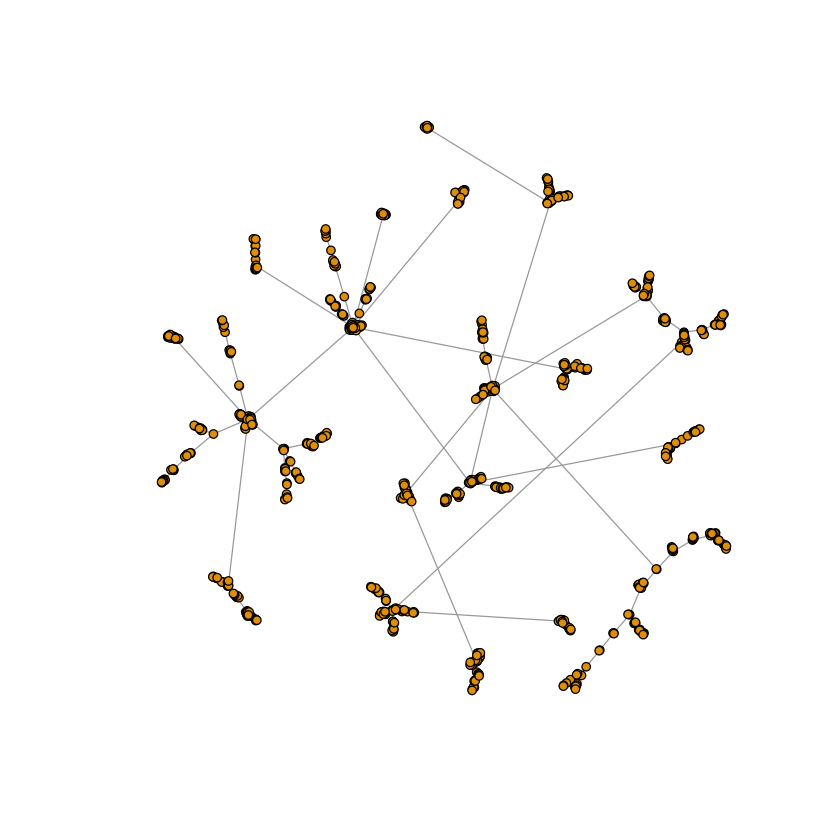
\includegraphics[width=0.5\textwidth]{1_2_a_network.png}
\caption{undirected graph with 1000 nodes based on preferential attachment Model}
\end{figure}

(b) We used fast greedy method to find the community structure. Mea- sure modularity.

\section{Random Walk on Networks}
\subsection{Random walk on Erdös-Rényi networks}
(a) Same as what we have done in the previous part, we generated an undirected random network containing 1000 nodes with the probability of 0.01 to add an edge between any pair of nodes. The graph we got is shown below:
\begin{figure}[H]
\centering
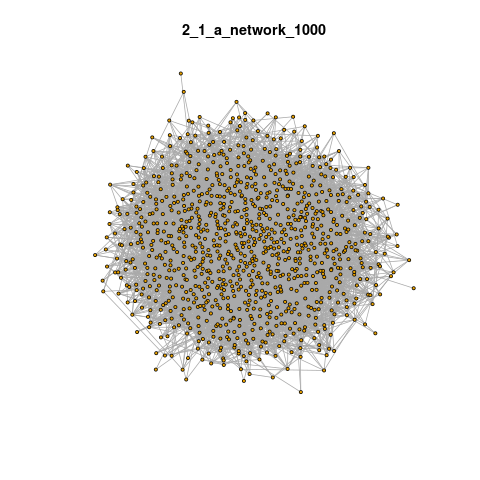
\includegraphics[width=0.5\textwidth]{2_1_a_network_1000.png}
\caption{undirected graph with 1000 nodes based on Erdös-Rényi Model}
\end{figure}

(b) After simulating random walk, we got following results:
\begin{figure}[htbp]
\centering
\begin{minipage}[t]{0.48\textwidth}
\centering
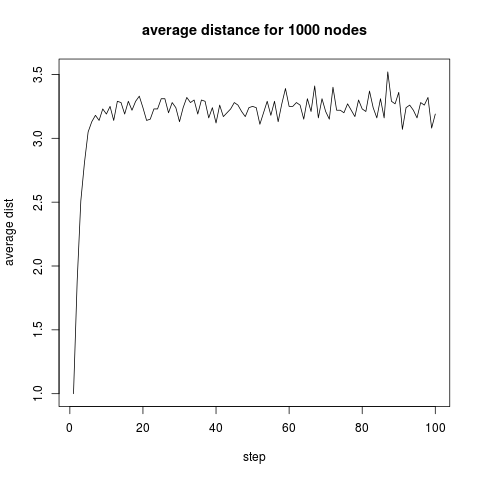
\includegraphics[width=7.5cm]{2_1_b_distance.png}
\caption{⟨s(t)⟩ v.s. t with nodes = 1000}
\end{minipage}
\begin{minipage}[t]{0.48\textwidth}
\centering
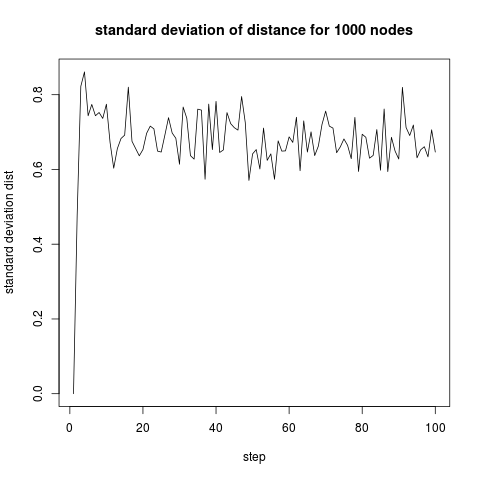
\includegraphics[width=7.5cm]{2_1_b_deviation.png}
\caption{σ2(t) v.s. t with nodes = 1000}
\end{minipage}
\end{figure}

(c) The degree distribution of the last reached nodes in N times of the random walk and the degree distribution of the graph are shown below.
\begin{figure}[htbp]
\centering
\begin{minipage}[t]{0.48\textwidth}
\centering
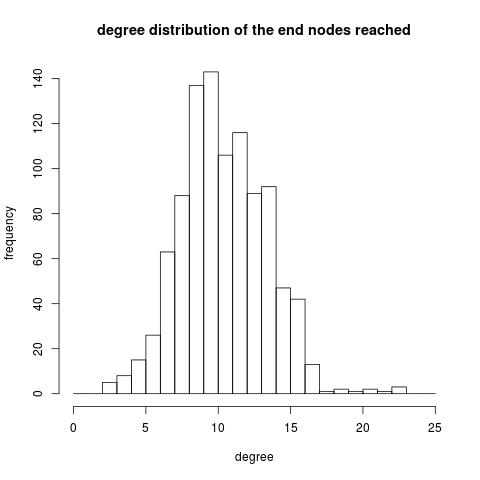
\includegraphics[width=7.5cm]{2_1_c_end_nodes_degree.png}
\caption{degree distribution of the ending node with nodes = 1000 in network}
\end{minipage}
\begin{minipage}[t]{0.48\textwidth}
\centering
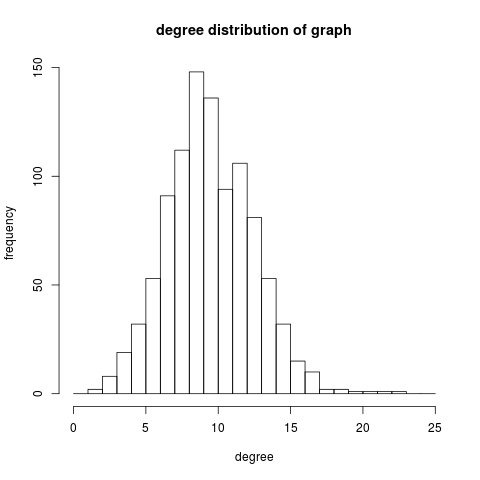
\includegraphics[width=7.5cm]{2_1_c_graph_degree.png}
\caption{degree distribution of the graph with nodes = 1000 in network}
\end{minipage}
\end{figure}

The results illustrate that the real graph degree distribution has similar trends with the degree distribution of the ending node by random walk. Both of them follows a Gaussian distribution. This could be proved by doing some simple calculation under the Erdös-Rényi Model. Every time a new node joins the network has the same probability (p) to add an edge to each existing nodes. That is to say, for all the nodes, the degree of a node follows binomial distribution. $$p_{k} = \qquad\mathrm{C}_{n-1}^k p^{k} (1-p) ^{n-1-k}$$ When the number of nodes (n) is large, Gaussian distribution could be seen the approximation of binomial distribution. 

(d) To figure out the difference of the shortest path length with different number of nodes in the network, we repeated what we have done in problem(b) under 100 nodes and 10000 nodes respectively in the network. Figure 6 and 7 show the average distance and standard deviation of distance under 100 nodes respectively, while figure 8 and 9 show the results under 10000 nodes.
The diameter of the nodes N = 100, N = 1000 and N = 10000 is about 2.0, 3.5 and 2.5 respectively. This seems not what we have expected, so we ran program several times to generate different networks with certain number of nodes. Not surprisingly, we found that graph with more nodes tend to have smaller diameter and smaller average distance. In addition, we can get another consequence from figures bellow that for the graph with 100 nodes, the average distance converge slowly or even cannot converge if we do not set the start node fixed. On the contrary, the results show less fluctuation with 10000 nodes. In conclusion, the smaller the diameter is, the average distance and standard deviation of the distance converge more quickly and turn out to have smaller fluctuation. 
\begin{figure}[htbp]
\centering
\begin{minipage}[t]{0.48\textwidth}
\centering
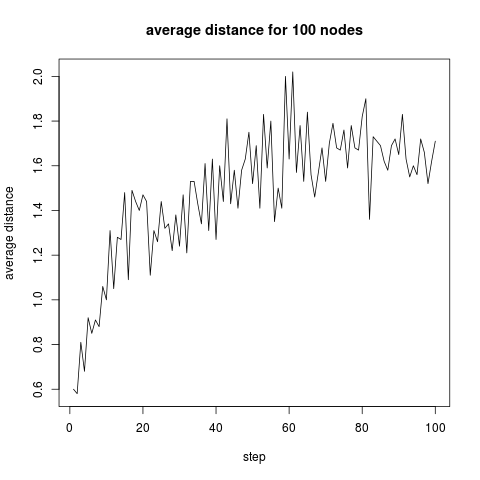
\includegraphics[width=7.5cm]{2_1_d_100_distance.png}
\caption{⟨s(t)⟩ v.s. t with nodes = 100}
\end{minipage}
\begin{minipage}[t]{0.48\textwidth}
\centering
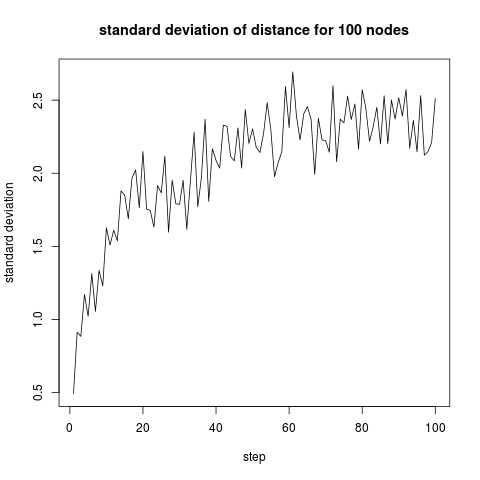
\includegraphics[width=7.5cm]{2_1_d_100_deviation.png}
\caption{σ2(t) v.s. t with nodes = 100}
\end{minipage}
\end{figure}
\begin{figure}[htbp]
\centering
\begin{minipage}[t]{0.48\textwidth}
\centering
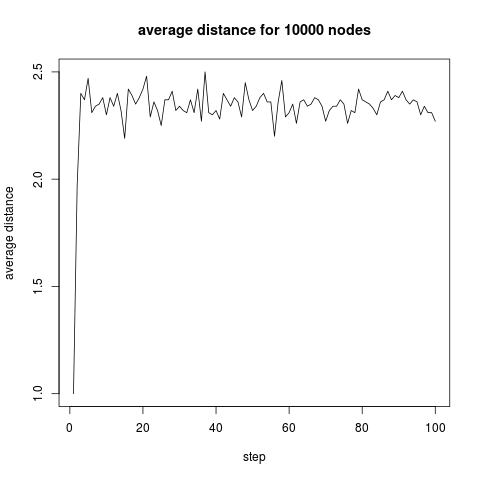
\includegraphics[width=7.5cm]{2_1_d_10000_distance.png}
\caption{⟨s(t)⟩ v.s. t with nodes = 10000}
\end{minipage}
\begin{minipage}[t]{0.48\textwidth}
\centering
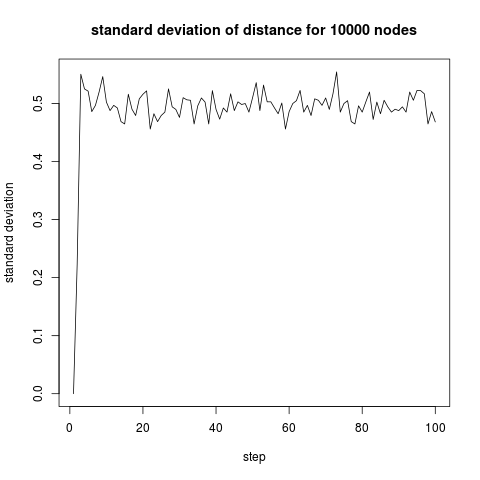
\includegraphics[width=7.5cm]{2_1_d_10000_deviation.png}
\caption{σ2(t) v.s. t with nodes = 10000}
\end{minipage}
\end{figure}

\subsection{Random walk on networks with fat-tailed degree distribution}
(a) We used function $sample_pa()$ to generate a fat-tailed network according to the Barabasi-Albert Model. The graph we got is shown bellow.
\begin{figure}[H]
\centering
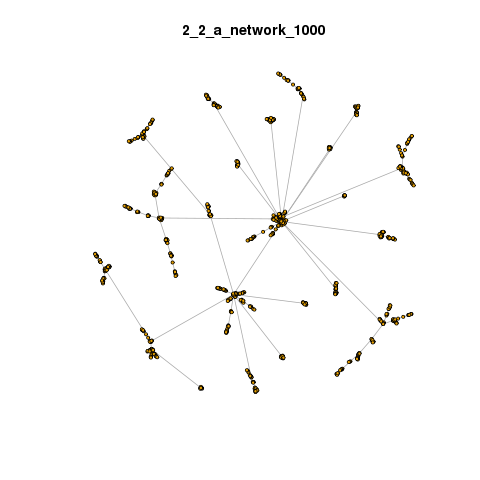
\includegraphics[width=0.5\textwidth]{2_2_a_network_1000}
\caption{undirected graph with 1000 nodes based on Barabasi-Albert Model}
\end{figure}

(b) As what we have dealt with Erdös-Rényi networks, we also simulated random walk on preferential attachment network and Figure 11 and 12 demonstrate the plot ⟨s(t)⟩ v.s. t and σ2(t) v.s. t respectively.
\begin{figure}[htbp]
\centering
\begin{minipage}[t]{0.48\textwidth}
\centering
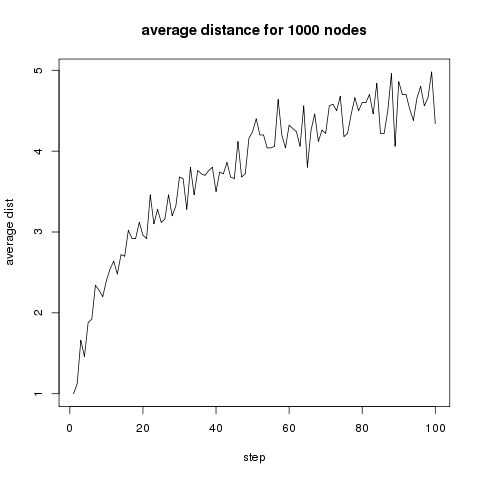
\includegraphics[width=7.5cm]{2_2_b_distance.png}
\caption{⟨s(t)⟩ v.s. t with nodes = 1000}
\end{minipage}
\begin{minipage}[t]{0.48\textwidth}
\centering
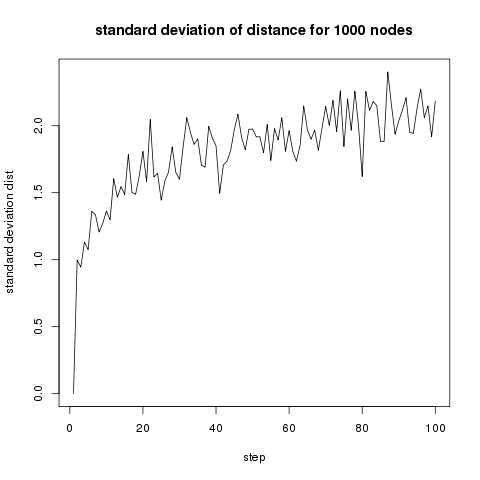
\includegraphics[width=7.5cm]{2_2_b_deviation.png}
\caption{σ2(t) v.s. t with nodes = 1000}
\end{minipage}
\end{figure}
(c) After running several times to get several figures(shown bellow), we could see that after a certain large number of steps of random walk, the results of two kinds of degree distribution are similar to each other.
\begin{figure}[htbp]
\centering
\begin{minipage}[t]{0.48\textwidth}
\centering
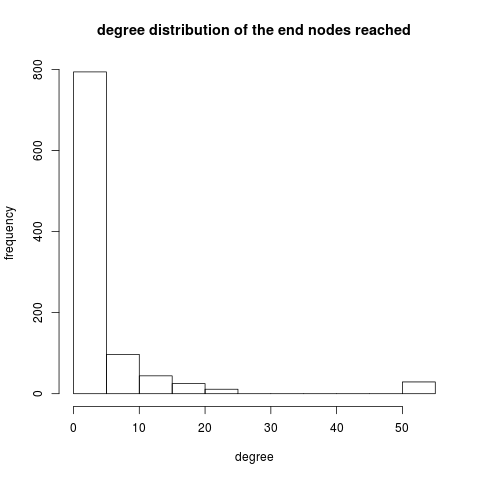
\includegraphics[width=7.5cm]{2_2_c_end_nodes_degree.png}
\caption{degree distribution of the ending node with nodes = 1000 in network}
\end{minipage}
\begin{minipage}[t]{0.48\textwidth}
\centering
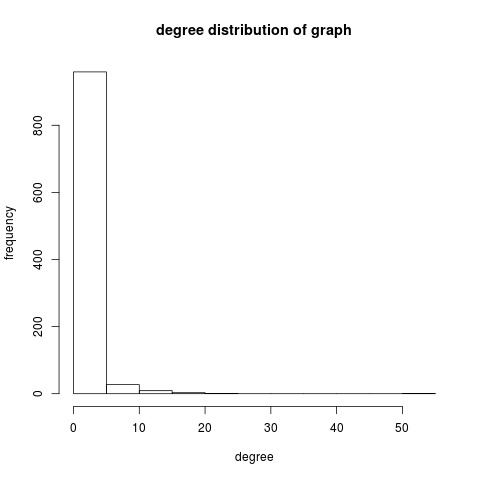
\includegraphics[width=7.5cm]{2_2_c_graph_degree.png}
\caption{degree distribution of the graph with nodes = 1000 in network}
\end{minipage}
\end{figure}

(d) Repeated the process in (b), we got the diameters of graphs with 100 and 10000 nodes are 4.5 and 5 respectively. Though we got this result, according to the theory, we knew that this seemed incorrect. Therefore, we generate network several times and calculate the average of the diameter. Then, we got the conclusion that in general, the graph with more nodes has smaller diameter, which means it also has smaller average distance.

The results also illustrate some differences between two different graph generation models. Considering the graph with 1000 nodes, in previous model(Erdös-Rényi Model), we can see that the average distance increases dramatically within not more than 10 steps, and then the value keeps fluctuating along the step t and gradually converges. However in Barabasi-Albert Model, the average distance shows a slight increase along the step t.
\begin{figure}[htbp]
\centering
\begin{minipage}[t]{0.48\textwidth}
\centering
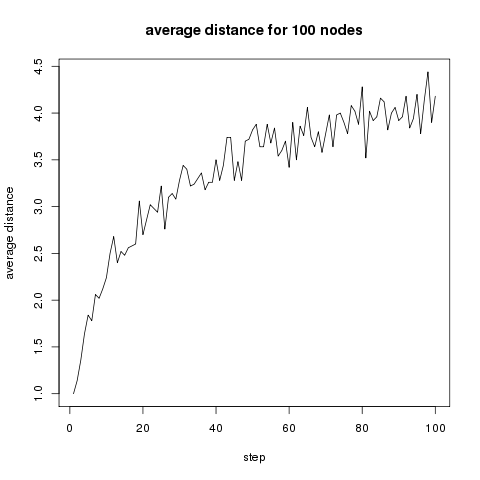
\includegraphics[width=7.5cm]{2_2_d_100_distance.png}
\caption{⟨s(t)⟩ v.s. t with nodes = 100}
\end{minipage}
\begin{minipage}[t]{0.48\textwidth}
\centering
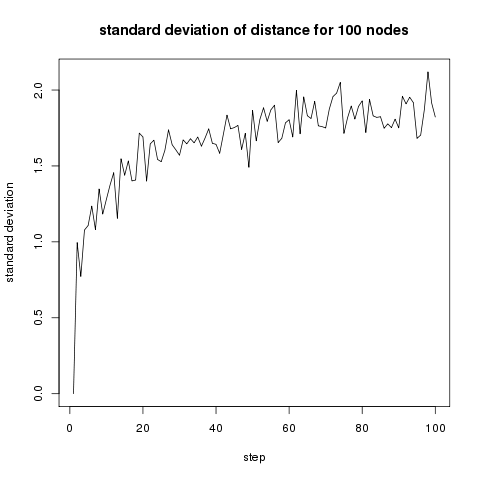
\includegraphics[width=7.5cm]{2_2_d_100_deviation.png}
\caption{σ2(t) v.s. t with nodes = 100}
\end{minipage}
\end{figure}
\begin{figure}[htbp]
\centering
\begin{minipage}[t]{0.48\textwidth}
\centering
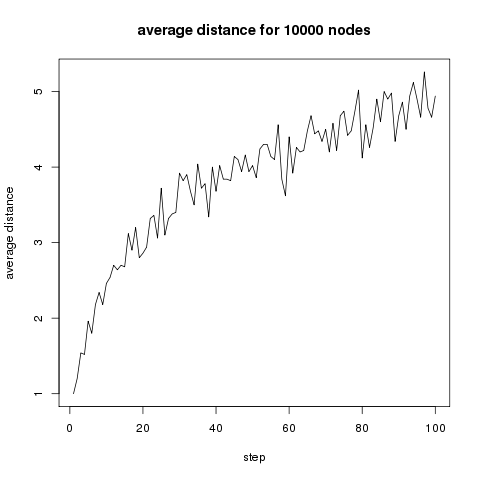
\includegraphics[width=7.5cm]{2_2_d_10000_distance.png}
\caption{⟨s(t)⟩ v.s. t with nodes = 10000}
\end{minipage}
\begin{minipage}[t]{0.48\textwidth}
\centering
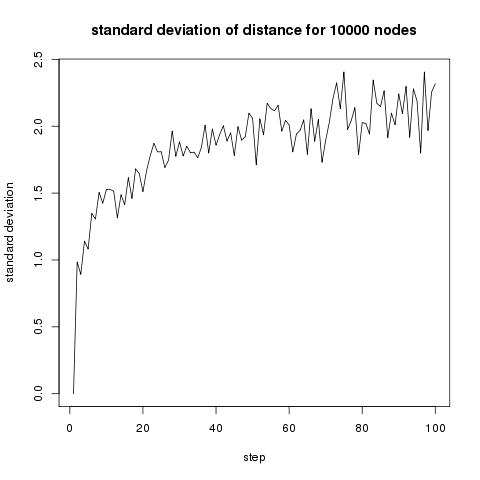
\includegraphics[width=7.5cm]{2_2_d_10000_deviation.png}
\caption{σ2(t) v.s. t with nodes = 10000}
\end{minipage}
\end{figure}



\subsection{PageRank}
PageRank is a famous algorithm designed by Larry Page, one of the founder of Google. Although there are a few limitations of this algorithm, many other ranking algorithms are invented under its inspiration. In this section, we applied random walk based on PageRank and got some interesting results which illustrate the principle of PageRank.

(a) The graph we generated based on preferential attachment is shown bellow. 
\begin{figure}[H]
\centering
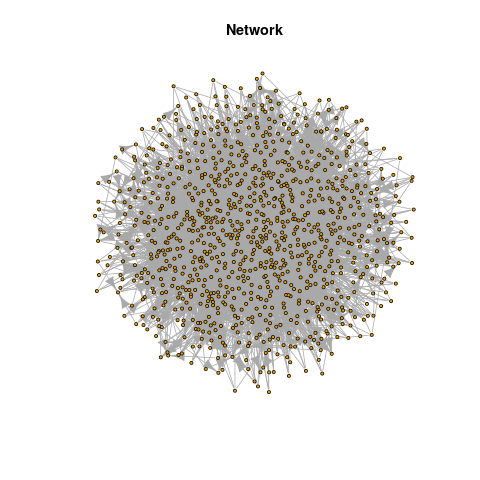
\includegraphics[width=0.5\textwidth]{3_network.png}
\caption{directed graph with 1000 nodes using preferential attachment }
\end{figure}
From the results shown bellow, it could be concluded that the visit probability is proportional to the node degree. The higher the node degree is, the more possible the walker would visit the node.
\begin{figure}[htbp]
\centering
\begin{minipage}[t]{0.48\textwidth}
\centering
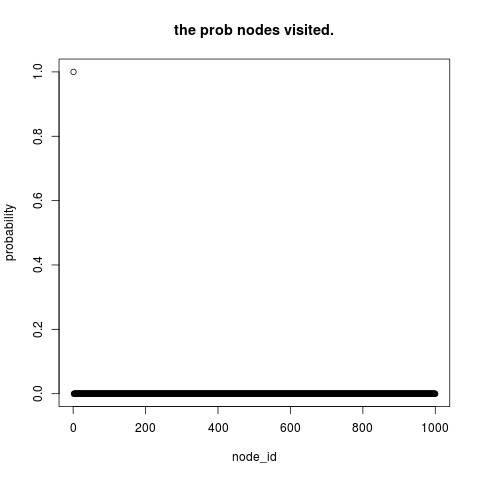
\includegraphics[width=7.5cm]{3_a_rw_prob.png}
\caption{probability that the walker visits each node}
\end{minipage}
\begin{minipage}[t]{0.48\textwidth}
\centering
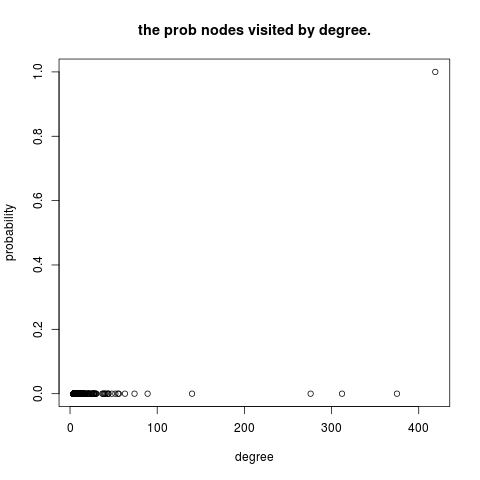
\includegraphics[width=7.5cm]{3_a_rw_prob_by_degree.png}
\caption{visit probability v.s. degree}
\end{minipage}
\end{figure}
(b) Considering the teleportation probability of $\alpha = 0.15$, we get slightly different results. 
\begin{figure}[htbp]
\centering
\begin{minipage}[t]{0.48\textwidth}
\centering
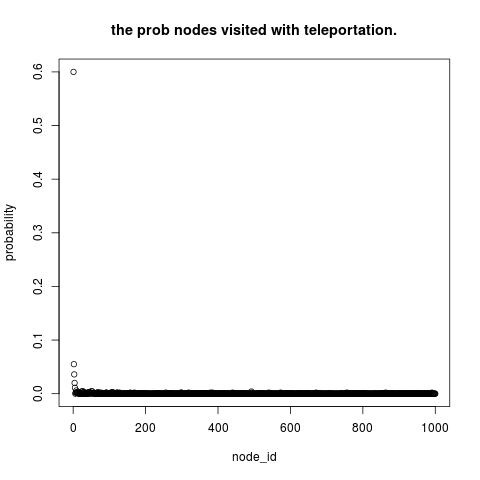
\includegraphics[width=7.5cm]{3_b_rw_prob_teleport.png}
\caption{probability that the walker visits each node with teleportation probability $\alpha = 0.15$}
\end{minipage}
\begin{minipage}[t]{0.48\textwidth}
\centering
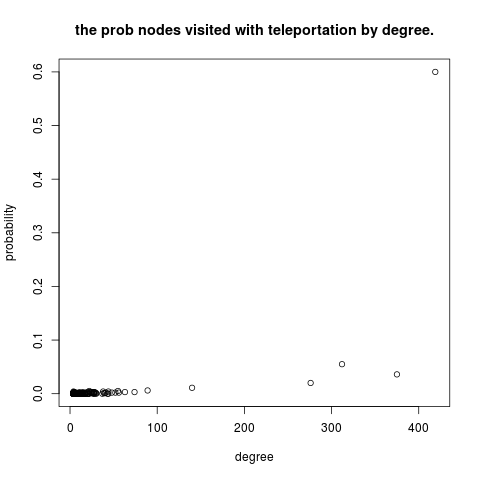
\includegraphics[width=7.5cm]{3_b_rw_prob_teleport_by_degree.png}
\caption{visit probability v.s. degree with teleportation probability $\alpha = 0.15$}
\end{minipage}
\end{figure}
It demonstrates that the difference of visiting probability along degree of the node is getting larger. 

\subsection{Personalized PageRank}
(a) In Personalized PageRank, we set the teleportation probability proportionally to PageRank of each node. The results are shown bellow.
\begin{figure}[htbp]
\centering
\begin{minipage}[t]{0.48\textwidth}
\centering
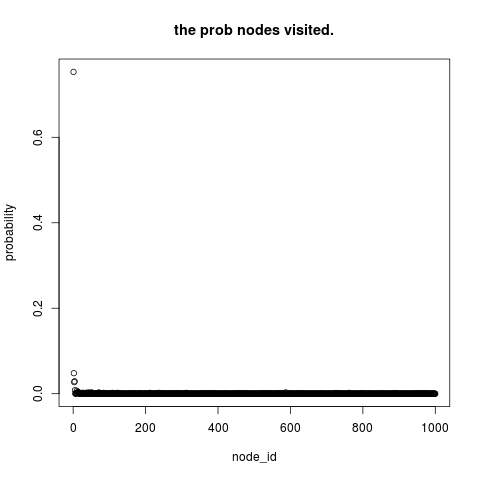
\includegraphics[width=7.5cm]{4_a_rw_prob.png}
\caption{probability that the walker visits each node under Personalized PageRank}
\end{minipage}
\begin{minipage}[t]{0.48\textwidth}
\centering
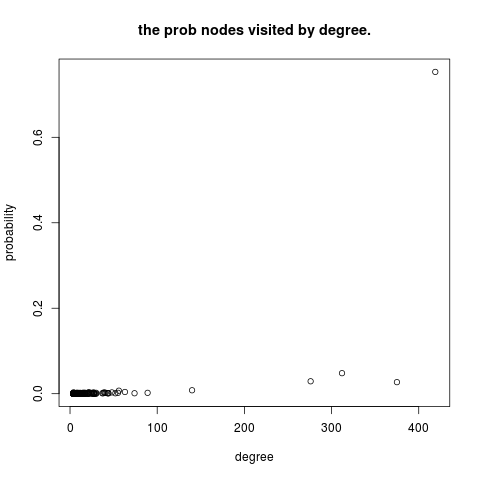
\includegraphics[width=7.5cm]{4_a_rw_prob_by_degree.png}
\caption{visiting probability v.s. degree under Personalized PageRank}
\end{minipage}
\end{figure}
Comparing to 3(a), the results show that Personalized PageRank can make degree of the node influence more to the visiting probability, which is in fact similar to what we get in 3(b). The higher degree the node is, the more possible it will be visited. In other words, since it is a preferential attachment model, the longer time a node stays in the network, the more possible it will be visited. 

(b) The results are shown bellow.
\begin{figure}[htbp]
\centering
\begin{minipage}[t]{0.48\textwidth}
\centering
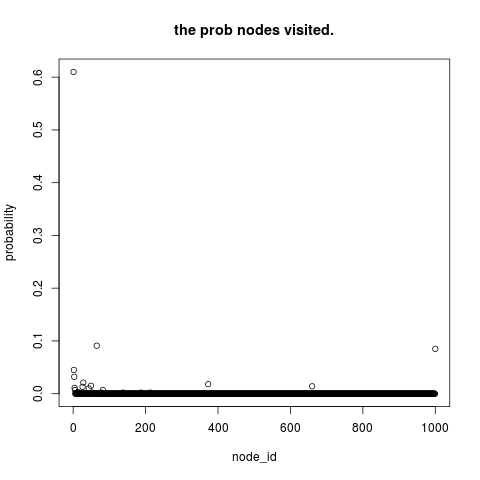
\includegraphics[width=7.5cm]{4_b_rw_prob.png}
\caption{probability that the walker visits each node under fixed teleportation}
\end{minipage}
\begin{minipage}[t]{0.48\textwidth}
\centering
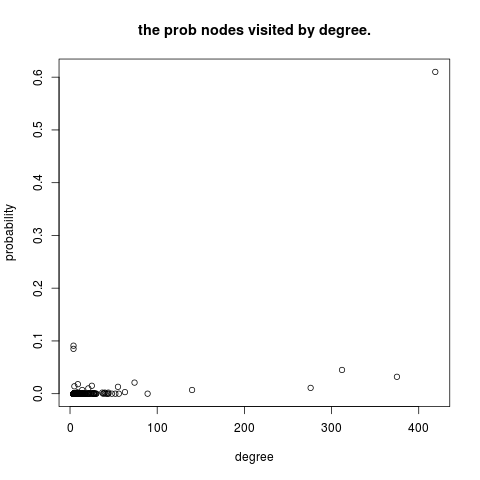
\includegraphics[width=7.5cm]{4_b_rw_prob_by_degree.png}
\caption{visiting probability v.s. degree under fixed teleportation}
\end{minipage}
\end{figure}
Comparing to all the results we get from PageRank or Personalized PageRank, under this circumstance, the visiting probability varies more significantly along the degree of a node. Specifically, some nodes with less than 100 degree have high probability to be visited than some other nodes with degree around less than 50. Nevertheless, this rarely happens in previous model, where nodes with degree of 300 or higher may be more possible to be visited than other nodes, while nearly most of nodes within the degree of 100 have similar visiting probability of around 0. Though it appears some irregular results within the degree of 100 (the visiting probability does not follow the rule exactly), the general rule that nodes with higher degree have more chance to be visited does not change. 
(c) Since at this time, nodes can only teleport to trusted nodes, which is similar to the previous problem that only two nodes are allowed to teleport to. Here, only the nodes belong to trusted node set are allowed to teleport to. Thus, the equation would be like this:
$$ r = \alpha \cdot T \cdot r + (1 - \alpha) \cdot d$$
where T is the transition matrix and vector d can be used to assign a non-zero score to the set of trusted pages only. In this way, trusted pages will have higher probability to be visited, and what these trusted pages point to can also be regarded as trustworthy pages, and their visiting probability will increase since we make restriction to teleport to trusted pages only. 



% that's all folks
\end{document}


